\documentclass{beamer}
\usetheme{CambridgeUS}
\usepackage[brazil]{babel}
\usepackage[utf8]{inputenc}
\useoutertheme{miniframes}
% \useoutertheme{tree}
  
\title{Aplicações de Treinamento Semi-Supervisionado em Casos Bipolares de Linguagem Natural}
%\stitle{SSL em PLN}
\subtitle{Trabalho final da da Matéria SCC5882, \\ {\bf Professores:} Dr. Zhao Liang e Dr. Alneu de Andrade Lopes}
\author[Renato Fabbri]{{\bf Aluno:} Renato Fabbri  \\ \texttt{renato.fabbri@gmail.com}}
\institute{IFSC-USP}

%\date
\begin{document}
  \frame{\titlepage}
  \section*{Sumário}
  \frame{\tableofcontents}
  \section{Introdução}
    \frame{\tableofcontents[current]}
    \subsection{Linguagem Natural}
%     \subsection{}
    \frame
    {
      \frametitle{Definição e suas Variações}
      \begin{itemize}
        \item Linguagem Natural: linguagem utilizadas normalmente por seres humando para se comunicarem.
        \item Em geral $\rightarrow$ Somente Conteúdo Textual.
        \item Processamento de Fala.
      \end{itemize}
    }

    \subsection{PLN e Processamento de Fala}
    \frame
    {
      \frametitle{PLN}
        \begin{itemize}
          \item Fonética e Fonologia - O estudo dos sons linguísticos.
          \item Morfologia - O estudo dos componentes das palavras (e seus significados).
          \item Sintáxe - O estudo da relação estrutural entre palavras.
          \item Semântica - O estudo dos significados.
          \item Pragmática - O estudo do uso da linguagem para fins específicos.
          \item Discurso - O estudo de unidades linguísticas que envolvem conjuntos de colocações, frases, etc.
        \end{itemize}
    }
    \frame
    {
      \frametitle{Processamento de Fala}
        \begin{itemize}
        \item Reconhecimento de Fala - lida com o a análise do conteúdo linguístico do sinal.
        \item Reconhecimento de Voz/Locutor - visa identificar o individuo que produz a fala.
        \item Codificação de voz - compactação de dados especializada.
        \item Análise de voz - fins médicos, estudos cognitivos, etc.
        \item Síntese de voz - fala artificial, geralmente gerada por computador.
        \item Melhora de fala - visa recuperar ou aumentar a inteligibilidade do sinal.
        \end{itemize}
    }


  \section{Extração de Características}
    \frame{\tableofcontents[current]}
    \subsection{Redes de Palavras}
      \frame
      {
        \frametitle{Formação (1)}
      \begin{figure}[!h]
        \begin{center}
                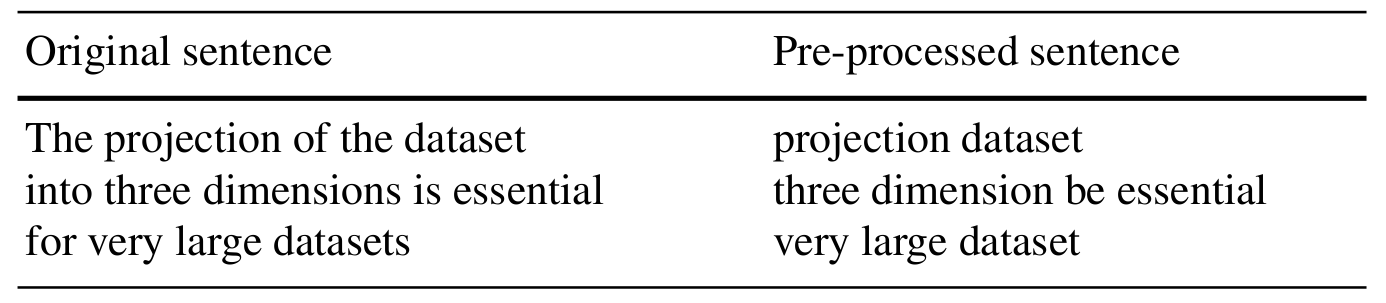
\includegraphics[width=.8\textwidth]{sentencas-processadas}
        \end{center}
        \caption{Processamento de texto para formação de redes complexas.}
      \end{figure}
      }

      \frame
      {
        \frametitle{Formação (2)}
      \begin{figure}[!h]
        \begin{center}
                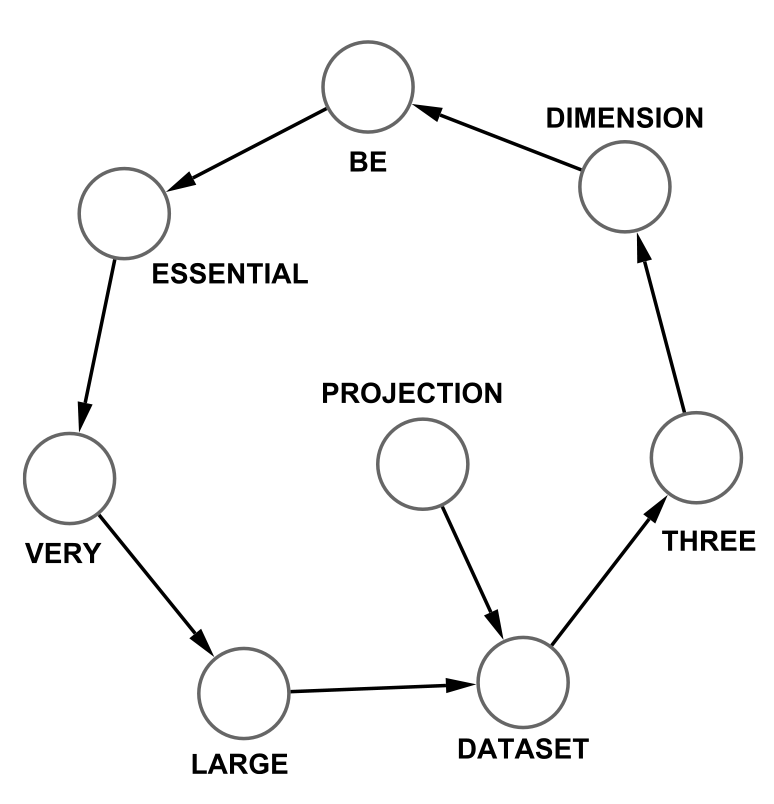
\includegraphics[width=.5\textwidth]{grafo-palavras}
        \end{center}
        \caption{Rede de palavras (excerto de rede).}
      \end{figure}
      }

      \frame
      {
        \frametitle{Formação - Caso Específico}
          \begin{itemize}
            \item Textos da Folha de São Paulo, coletados por 10 anos.
            \item Opiniões negativas e positivas.
            \item Textos aglomerados até atingirem 1200 vértices.
            \item Extraímos as medidas de cada aglomerado: graus, coeficientes de clusterização, caminhos mais curtos, eficiência global, proximidade(closeness) e acessibilidade.


        \end{itemize}
      }

   \subsection{Processamento de Fala}
      \frame
      {
        \frametitle{Atributos - Método Geral}
          \begin{itemize}
          \item Medidas estatísticas
          \item Frequência Fundamental.
          \item Amplitude/Intensidade/Energia.
          \item Harmônicos.
          \item Articulação.
          \item Pausas.
        \end{itemize}
      }

      \frame
      {
        \frametitle{Atributos}
          \begin{itemize}
          \item Frequência fundamental a cada 0.01 segundo.
          \item Média, desvio padrão, âmbito, mediana, abaixo do limiar, acima do limiar.
          \item Praat e Python.
        \end{itemize}
      }

   \subsection{Tratamento dos Dados}
      \frame
      {
        \frametitle{Normalização e PCA}
          \begin{itemize}
          \item (medida - média) / desvio padrão
          \item PCA
        \end{itemize}
      }

  \section{Reconhecimento de Padrões}
    \frame{\tableofcontents[current]}
    \subsection{Tradicionais}
      \frame
      {
        \frametitle{Métodos Utilizados (Confronto)}
        \begin{itemize}
          \item Bayesian Decision
          \item Decision Tree
          \item Decision Rules
          \item Naive Bayes
        \end{itemize}
      }
    \subsection{SSL}

      \frame
      {
        \frametitle{Propagação de Rótulo - Concepção}
        \begin{itemize}
          \item Vizinho mais próximo $\rightarrow$ propaga mais fácil.
          \item Rótulos fixos nos rotulados de antemão.
          \item Estes "emanam" rótulos.
        \end{itemize}
      }

      \frame
      {
        \frametitle{Convenções e Exposição do Problema}
        \begin{itemize}
          \item ${(x_1,y_1)...(x_l,y_l)}$ os dados rotulados.
          \item $y \in {1...C}$ com $C$ o número de classes.
          \item ${x_{l+1}...x_{l+u}}$.
          \item Seja $n = l + u$
          \item L e U denotam os dados rotulados e não rotulados, respectivamente
        \end{itemize}
      }

      \frame
      {
        \frametitle{Obtenção do Grafo}
        \begin{itemize}
          \item Completo.
          \item $w_{ij} = exp( -\frac{\| x_i - x_j \|^2}{\alpha^2} )$
          \item $\alpha$ é um \emph{hiperparâmetro}
        \end{itemize}
      }  

      \frame
      {
        \frametitle{Matriz de Transição}
        \begin{itemize}
          \item $P_{ij}$ é a probabilidade de transição do nó $i$ para o nó $j$ (passagem do rótulo)
          \item $P_{ij} = P(i \rightarrow j) = \frac{w_{ij}}{\sum_{k=1}^{n}w_{ik}}$
        \end{itemize}
      }

      \frame
      {
        \frametitle{Últimas Definições}
        \begin{itemize}
          \item Matriz de rótulos $Y_L$, $l \times C$, cuja \emph{iésima} linha possui $1$ na coluna correspondente à classe do dado $x_i$.
          \item $f$ uma matriz $n \times C$ em que cada linha pode ser interpretada como uma distribuição de probabilidade sobre os rótulos.
        \end{itemize}
      }
      \frame
      {
        \frametitle{Implementação do Algoritmo de Propagação de Rótulo}
\begin{equation}
  f_u = (I - P_{UU})^{-1}P_{UL}Y_{L}
\end{equation}

        \begin{center}
        implementação $\rightarrow$ algoritmos/ssl-propagacao-de-rotulo.py
        \end{center}
      }

      \frame
      {
        \frametitle{Mincut - Concepção e Implementação}
        \begin{itemize}
          \item Objetos parecidos devem ficar juntos.
          \item Seccionamento por separações de custos mínimos.
        \end{itemize}

        \begin{center}
implementação $\rightarrow$ algoritmos/ssl-mincut.py
        \end{center}
      }

  \section{Resultados}
    \frame{\tableofcontents[current]}
    \subsection{Redes de Palavras}
      \frame
      {
        \frametitle{Métodos Tradicionais}
      \begin{figure}[!h]
        \begin{center}
                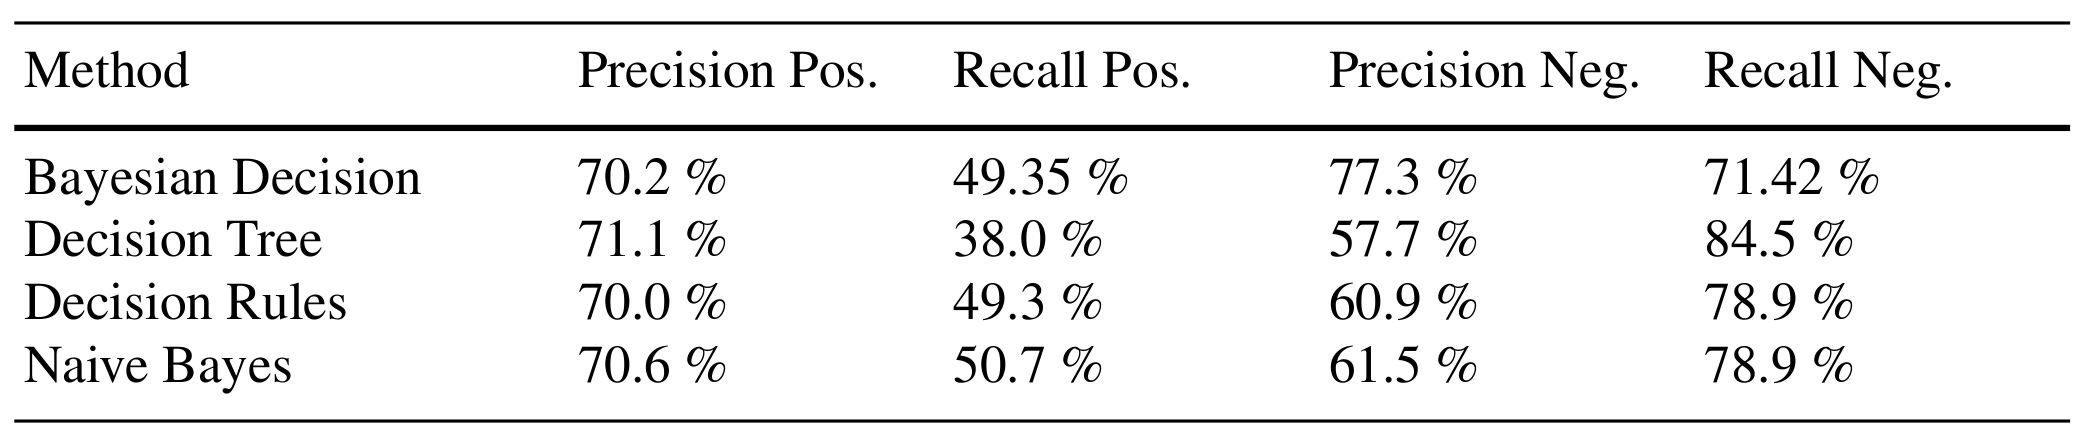
\includegraphics[width=.7\textwidth]{palavras-diego}
        \end{center}
        \caption{Reconhecimento de polaridades via métodos tradicionais.}
      \end{figure}
      }
      \frame
      {
        \frametitle{Propagação de Rótulo}
        \begin{center}
            NA MONOGRAFIA (era texto/resultados/*)
        \end{center}
      }
    \subsection{Processamento de Fala}
      \frame
      {
        \frametitle{Métodos Tradicionais}
        \begin{center}
            NA MONOGRAFIA (era audio/trad/*)
        \end{center}
      }
      \frame
      {
        \frametitle{Propagação de Rótulo}
        \begin{center}
            NA MONOGRAFIA (era audio/resultados/*)
        \end{center}
      }

  \section{Discussão e Desenvolvimentos Futuros}
    \frame{\tableofcontents[current]}
    \frame
    {
      \frametitle{Discussão dos Resultados}
      \begin{itemize}
        \item Resultados melhores para os casos que estudamos (se comparado aos métodos de treinamento supervisionado tradicionais)
        \item Maior variedade de taxas de acertos dependendo do conjunto de objetos escolhidos.
        \item Destaque para a utilização de várias amostras (em contraste com o que a literatura salienta).
      \end{itemize}
    }

    \frame
    {
      \frametitle{Desenvolvimentos Futuros}
      \begin{itemize}
        \item Afinar a extração de características (limiar utilizado só recentemente).
        \item Redes de Prosódia, visibilidade e seccionamento do espectro.
        \item Em conjunto com os métodos já utilizados, empregar a \emph{Propagação de Rótulo} nos trabalhos.
      \end{itemize}
    }

  \section{Disponibilização}
    \frame{\tableofcontents[current]}
    \frame
    {
      \frametitle{Na Rede}
      \begin{itemize}
        \item svn co http://svn.assembla.com/svn/audioexperiments/NinjaML
      \end{itemize}
    }
  \section{Bibliografia Principal}
    \frame{\tableofcontents[current]}
    \frame
    {
      \frametitle{Referências Principais}
      \begin{itemize}
        \item Zhu, X. and Lafferty, J. and Rosenfeld, R. "Semi-supervised learning with graphs.", 2005
        \item Zhu, X. and Ghahramani, Z., "Learning from labeled and unlabeled data with label propagation.", 2002
        \item Blum, A. and Chawla, S., "Learning from labeled and unlabeled data using graph mincuts", 2001
        \item (Mais detalhes na monografia)
      \end{itemize}
    }
%     \frame
%     {
%       \frametitle{Esquema Geral}
%       \begin{figure}[!h]
%         \begin{center}
%                 \includegraphics[width=1\textwidth]{3000-series}
%         \end{center}
% %         \caption{}
%       \end{figure}
%     }

\end{document}
